\chapter{Maximum entropy principle}
\label{chap:maximum_entropy_principle}
\section{Introduction}
When rolling a fair six-sided dice $N$ times, there are a total of $E = 6$ distinct outcomes, each corresponding to one of the six faces of the dice. In the absence of any additional information, the Principle of Insufficient Reason (also known as the Principle of Indifference) can be applied. This principle suggests that if there are $n$ possibilities that are indistinguishable except for their names, then each of these possibilities should be assigned a probability equal to $1/n$. This approach is historically associated with mathematicians such as J. Bernoulli, Laplace, and Keynes.\\
However, when new information or constraints are introduced, the challenge becomes assigning probabilities to the $E$ outcomes in a way that satisfies these constraints without making any unwarranted additional assumptions. In other words, the goal is to update the probability distribution over the outcomes based on the available information while avoiding any biases or unsupported assumptions. This process is fundamental in Bayesian probability theory, where prior probabilities are updated with new evidence to arrive at posterior probabilities that reflect the updated state of knowledge.\\
Let $\vec{n} =(n_1,\ldots,n_E)$ denote a situation in which the $N$ realizations yield $n_i$ instances of outcome $i$. The number of possible outcomes of the $N$ realizations is $E^N$, the nu,ber corresponding to $\vec{n} = (n_1,\ldots,n_R)$ is:
\[
W(\vec{n})
 = \frac{N!}{\prod_{i=1}^{E} n_i!}
\]
with the constraint
\[
\sum_{i=1}^{E} n_i = N
\]
the interchanges within the same outcome are unobservable.\\
When $n_i$ are large, we can use Stirling's approximation, and in the limit $N \to \infty$ we obtain:
\[
\frac{\ln W (\vec{n})}{N} \to - \sum_i P_i \ln P_i \equiv H(\vec{P})
\]
where $P_i$ is the frequency of the occurrence of the $i$th event:
\[
P_i = \frac{n_i}{N}
\]
and $H$ is the entropy of the distribution probability $\vec{P} = (P_1,\ldots,P_E)$
\section{Maximum entropy solution}
Repeating the experiment $N$ times, the distribution $\vec{n} = N\vec{P}$ is proportional to:
\[
W(\vec{n}) \propto \exp(NH(\vec{P}))
\]
The most probable $\vec{n} = (n_1,\ldots,n_E)$ among the total number of conceivable distinct results of the oucome of all $N$ realization is obtained by the maximization program:
\[
\vec{P}^* = \arg\max H(\vec{P}) \qquad \text{s.t.} \sum_{i=1}^{E}P_i = 1
\]
The solution is:
\[
P_i = \frac{1}{E}
\]
We can add more constraints in order to limit the range of possible $\vec{P}_s$. Constraints can be often be casted in terms of averages of certian quantities, for exemple given a quantity $Q$, known the value $Q_i$ of single outcome and known the average $\bar{Q}$, we have:
\[
\expected{Q} \equiv \sum_{i=1}^{E} P_i Q_i = \bar{Q}
\]
We can solve this problems through Lagrange multipliers:
\[
\mathcal{L} \equiv - \sum_i P_i \ln P_i - \alpha \sum_i P_i - \beta \sum_i P_iQ_i
\]
Derivate we obtain:
\[
P_i = \exp [-1-\alpha -\beta Q_i]
\]
so that $\sum_{i=1}^{E} P_i =1$, we obtain:
\[
P_i = e^{-\beta Q_i}/Z
\]
with
\[
Z = \sum_i e^{-\beta Q_i}
\]
is the partition function. Imposing the constraint $\sum_{i=1}^E P_iQ_i = \bar{Q}$ we obtain the value of $\beta$ solving the problem.\\
The compact form is:
\[
\bar{Q} = - \frac{1}{Z} \frac{\partial Z}{\partial \beta} = - \frac{\partial \ln Z}{\partial \beta}
\]
Taking several constraint, so that $\bar{Q}_a = -\partial \ln Z/ \partial \beta_a$ and taking the second derivate of log-partition, we obtain:
\begin{align*}
\frac{\partial^2 \ln Z}{\partial \beta_a^2} = \ldots = \overbrace{\expected{Q_a^2} - \expected{Q_a}^2}^{\text{variance}}\\
\frac{\partial^2 \ln Z}{\partial \beta_a \partial \beta_b} = \ldots = \underbrace{\expected{Q_a,Q_b} - \expected{Q_a}\expected{Q_b}}_{\text{covariance}}
\end{align*}
We can rewritten the first relation as:
\begin{mytheorem}[Fluctuation-dissipation theorem]
\[
Var[Q_a] = -\frac{\partial \expected{Q_a}}{\partial \beta_a}
\]
\end{mytheorem}
Summarizing:
\[
-\nabla_{\vec{\beta}}\ln Z = \expected{\vec{Q}} \qquad H_{\vec{\beta}}(\ln Z) = Cov[\vec{Q}]
\]
where $H_{\vec{\beta}}(Z)$ is the Hessian of the partition function.
\section{Maximum entropy for networks}
The Maximum Entropy Principle is a concept that has been widely applied in the field of network theory. The fundamental idea behind its application is to construct ensembles of networks while imposing specific constraints or properties on those networks.
Here's how the principle is applied:
\begin{itemize}
\item Observing a Network: Initially, one observes a single realization of a network and measures various observables or characteristics of that network. These observables could include properties like network density, node degrees, clustering coefficients, and other network metrics.

\item Assumption of an Ensemble: The key assumption is that the observed network is a particular realization of a larger ensemble of networks. This ensemble is defined in such a way that the average values of the observables in the ensemble are equal to the values observed in the data.
\end{itemize}
We consider two kind of ensemble, depends on how constraints are preserved:
\begin{itemize}
	\item Microcanonical: the constraints are preserved;
	\item Canonical: the constraint are preserved on average
\end{itemize}
\subsection{Microcanonical ensemble}
In the microcanonical ensemble the constraints are preserved exactly, i.e. each member of the ensemble satisfies the constraints. In the microcanonical ensemble all the realizations have the same probability. The
probability of a graph $G_i$ is:
\[
P(G_i) = \frac{1}{\mathcal{N}}
\]
where $\mathcal{N}$ is the number of possible graphs satisfying all the constraints, but often it is really hard count how many configurations.Few cases are analytically solvable: random graph and bipartite networks.\\
Numerical simulations to generate the microcanonical ensemble of the configuration model of a binary network are based on the local rewiring algorithm, where each individual move (rewiring) preserves the degree of the four involved nodes:
\begin{center}
	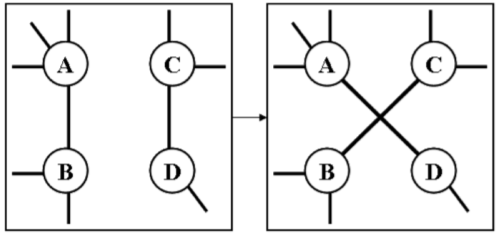
\includegraphics[width=0.5\textwidth]{picture/(43)local_rewiring.png}
\end{center}
By simulating a large number of networks with the local rewiring algorithm one creates an ensemble of graphs where the degree sequence is exactly the same as the original one. One can measure the empirical expected number $\expected{K}$ and the empirical standard deviation $\sigma[K]$ of the observed number $K$ of a specific motif in the simulated networks of the ensemble, and then compute the $z$-score:
\[
z = \frac{K_t - \expected{K}}{\sigma[K]}
\]
where $K_t$ is the nu,mber of motifs observed in the real word
\section{Exponential Random Graphs}
Let consider the simplest case of uniderected and unweighted newtork (withou selfloops) and consider $\mathcal{G}$ the set of graphs. Taken $G\in \mathcal{G}$ and be $P(G)$ the probability of that graph in our ensemble. Suppose we have a collection of graph observables $\{x_i\}, i =1,\ldots,r$ and suppose to have an estimane $\langle x_i \rangle$. Probability distribution for $G$ is done by maximizing Gibss entropy:
\[
S = - \sum_{G \in \mathcal{G}} P(G) \ln P(G)
 \]
subject to the constraint:
\[
\sum_G P(G) x_i(G) = \langle x_i \rangle
\]
and normalization condition:
\[
\sum_G P(G) =1
\]
Introducing the Lagrange multipliers $\alpha, \{\theta_i\}$we and solving the minimization, we found:
\[
P(G) = \frac{e^{-H(G)}}{Z}
\]
where the graph Hamiltonian is:
\[
H(G) = \sum_i \theta_ix_i(G)
\]
and partition function:
\[
Z =\sum_G e^{-H(G)} = e^{\alpha + 1}
\]
these equations define the exponential random graph model. Supposing the know the expected number od edges$\langle m \rangle$ of the network, the Hamiltonian is:
\[
H(G) = \theta m(G)
\]
since the number of edge of a graph $G$ is $m = \sum_{i<j} a_{ij}$, partition function is:
\[
Z = \sum_Ge^{-H} =\ldots = \prod_{i<j} \left(1 + e^{-\theta}\right) = [1 + e^{-\theta}]^{n \choose 2}
\]
The free energie defined as $F = - \ln Z$, we have:
\[
F = - {n \choose 2} \ln (1+ e^{-\theta})
\]
The expected number of edges is:
\[
\langle m\rangle = \frac{\partial F}{\partial \theta} = {n \choose 2}\frac{1}{e^\theta +1}
\]
we can re-parametrizes:
\[
p =\frac{1}{e^{\theta} + 1}
\]
so $\langle m \rangle = {n \choose 2}p$
The probability $P(G)$ of the ensemble is:
\[
P(G) -\frac{e^{-H}}{Z} = \ldots = p^m(1-p)^{{n \choose 2} -m}
\]
some comments:
\begin{itemize}
	\item $P(G)$ is constant
	\item $P(G)$ is simply the probability for a graph in which each of the ${n \choose 2}$ edges are present with probability $p$
	\item In graph theory this model is Erd\"os-Reny graph
	\item Due to independence, degree distrbution is binomial (or Poisson for large $n$)
\end{itemize}
The random graph is unrealistic null model for real network (most of the times, degree distribution in scale-free). A more realsitic model is imposing the full degree sequence $\{k_i\}_{i =1,\ldots,n}$. The Hamiltonian is:
\[
H = \sum_i \theta_i k_i
\]
with $n$ Lagrange multipliers $\theta_i$. Since $k_i = \sum_j a_{ij}$, the Hamiltonian becomes:
\[
H = \sum_{ij} \theta_i a_{ij} = \sum_{i<j} (\theta_i + \theta_j)a_{ij}
\]
partition function is:
\[
Z = \sum_{\{a_{ij}\}} \exp \left[- \sum_{i<j}(\theta_i + \theta_j)a_{ij}\right] = \ldots = \prod_{i<j} (1 + e^{- (\theta_i + \theta_j)})
\]
This model is a special case of an Hamiltonian:
\[
H = ]sum_{i<j} \Theta_{ij}a_{ij}
\]
any Hamiltonian where the link value is assigned, the configuration model corresponds to $\Theta_{ij} = \theta_i + \theta_j$ (random graph corresponds to $\Theta_{ij} =1$). The general case is:
\[
Z = \prod_{i<j} (1 + e^{-\Theta_{ij}}) \qquad F = - \sum_{i<j} \ln (1 + e^{- \Theta_{ij}})
\]
probability $p_{ij}$ of occurrence of an edge can be computed as:
\[
p_{ij} = \frac{1}{e^{\Theta_{ij}} + 1}
\]
SO that partion function factorizes implies we can calculate the probability of a graph:
\[
P(G) = \frac{e^{-H(G)}}{Z} =\ldots = \prod_{i<j} \frac{e^{- \Theta_{ij}a_{ij}}}{1 + e^{- \Theta_{ij}}}
\]
we can rewrite $P(G) = \prod_{i<j} q_{ij}$, where:
\[
q_{ij} = p_{ij}^{a_{ij}}(1-p_{ij})^{(1-a_{ij})}
\]
as product of independe Bernoulli variables, with:
\[
p_{ij} = \frac{e^{-\Theta_{ij}}}{1 + e^{- \Theta_{ij}}}
\]
In configuration model:
\[
p_{ij} = \frac{e^{- \theta_i - \theta_j}}{1 + e^{-\theta_i - \theta_j}}
\]
setting $b_i \equiv e^{-\theta_i}$ we obtain:
\[
p_{ij} = \langle a_{ij} \rangle = \frac{b_ib_j}{1 + b_i b_j}
\]
At the end, we can evaluate the expectation values of any product of vertex degree as:
\[
\langle k_ik_j\ldots \rangle = \frac{1}{Z} \left[\frac{\partial}{\partial \theta_i}\frac{\partial}{\partial \theta_j}\ldots\right]Z
\]
For example we obtain:
\begin{align*}
&\langle k_ik_j \rangle_c = Cov[k_ik_j] = \frac{\partial^2 F}{\partial \theta_i \partial \theta_j} = \frac{e^{\theta_i + \theta_j}}{(e^{\theta_i + \theta_j} +1)^2} \qquad i\neq j \\
& \langle k_i^2 \rangle_c = Var[k_i] = (n-1)\frac{e^{2\theta_i}}{(e^{2\theta_i}+1)^2}
\end{align*}
\subsection{The weighted configuration model}
Supposing weighted graph, with $w_{ij} \in \mathcal{N}$, we want to construct the maximum entropy ensemble of networks, we impose $\{s_i\}_{i=1,\ldots,n}$ where $s_i = \sum_{i\neq j} w_{ij}\in \mathbb{N}$
The Hamiltonian is:
\[
H = \sum_i \theta_i s+i
\]
with $n$ Lagrange multipliers $\theta_i$
Partition function is:
\[
Z = \prod_{i<j} \frac{1}{1 - e^{-(\theta_j + \theta_i)}}
\]
this can be easily generalized to the Hamiltonian:
\[
H = \sum_{i<j}\Theta_{ij} w_{ij}
\]
the average weight between nodes $i$ and $j$ is:
\[
n_{ij} = \langle w_{ij} \rangle = \frac{\partial F}{\partial \Theta_{ij}}
 = \frac{1}{e^{\Theta_{ij}}-1}
\]
We notice that this quantity diverges when $\Theta_{ij} ]\to 0$ (in Statistical mechanics this is colled as Bose-Einsten condensation), For the pure weighted configuration model:
\[
n_{ij} = \frac{1}{e^{\theta_i + \theta_j} - 1}
\]
and for weighted random graph:
\[
n_{ij} = \frac{1}{e^\theta -1}
\]

There exists a direct analogy between binary network statistics and Bose-Einstein statistics, as well as between weighted network statistics and Fermi-Dirac statistics. To understand this analogy, it's helpful to draw parallels with quantum statistical mechanics:
\begin{itemize} 
\item Binary Networks and Bose-Einstein Statistics: In binary networks, the analogy is akin to bosons in quantum mechanics. Bosons are particles that can occupy the same quantum state without limit. In binary networks, nodes or elements can share the same state or connection. For instance, in a social network, multiple individuals can be connected to a common friend without constraints.

\item Weighted Networks and Fermi-Dirac Statistics: Weighted networks have an analogy with Fermi-Dirac statistics. Fermions are particles that obey the Pauli exclusion principle, which means that only one particle can occupy a given quantum state at a time. In weighted networks, the weights on edges or connections can represent exclusive occupancy, such as in transportation networks where a single vehicle can occupy a specific route at a time.
\end{itemize}
The statistical mechanics ensembles of bosons or fermions are derived by solving the maximization problem:
\begin{align*}
	&\arg\max \left(-k_N \sum_\nu P(\nu) \ln P(\nu)\right)\\
	\text{s.t.} \quad \sum_\nu P(\nu) =1 \quad &\sum_\nu P(\nu)E(\nu) = \langle E \rangle \quad \sum_\nu P(\nu)N(\nu) = \langle N \rangle
\end{align*}
where $E(\nu)$ and $N(\nu)$ is the energy and the number of particle in quantum state $\nu$.\\
For bosons $N(\nu)$ runs from $0$ to $\infty$m while fermions runs from $0$ to $1$, using Langrange multipliers for bosons:
\[
Z = \prod_{i} \left[\frac{1}{1 - e^{-\beta(\epsilon_i - \mu)}}\right] \qquad \langle n_i \rangle =\frac{1}{e^{\beta(\epsilon_i - \mu)}-1}
\]
and for fermions:
\[
Z = \prod_i [1 + e^{-\beta (\epsilon_i - \mu)}] \qquad \langle n_i \rangle = \frac{1}{e^{\beta (\epsilon_i - \mu)}+1}
\]
where $\mu$ is a Lagrange multiplier (chemical potential in physics) and $\beta \equiv 1/k_BT$ in another multiplier (and $T$ is the temperature). \\ 
So that binary ensembles of networks are called fermionic and weighted ensembles of networks are called bosonic.
\section{Maximum likelihood and entropy}
The maximum entropy method gives the probabilities of an ensemble of networks depending on a vector of parameters (the Lagrange multipliers):
\[
P(G| \vec{\theta}) = \frac{e^{- H(G)}}{\sum_{G'} e^{-H(G')}} = \frac{e^{-\sum_i \theta_i x_i(G)}}{\sum_{G'} e^{- \sum_i \theta_i x_i(G)}} = \exp[-\vec{\theta} \cdot \vec{x}(G) - \ln Z (\vec{\theta})]
\]
The log-likelihood function is:
\[
\mathcal{L}(\vec{\theta})\equiv \ln P(G| \vec{\theta}) = - \sum_i \theta_ix_i(G) - \ln Z(\vec{\theta})
\]
In order to obtain the Lagrange multipliers, we can maximize the log-likelihood:
\begin{itemize}
\item Given a real network $G^{\ast}$ 
\item Choose the null model and measures the corresponding constraints in $G^\ast$ 
\item Build the ensemble by using maximum entropy and the constraints to obtain $P(G^\ast|\vec{\theta})$
\item (Numerically) determine the parameters $\vec{\theta}$ by maximizing the log-likelihood
\end{itemize}
It can be demonstrated straightforwardly that the parameters (denoted as $\theta^\ast$) that maximize the log-likelihood in a network model are chosen in such a way that the constraints used in the maximum entropy step, which defines the ensemble, ensure that the desired constraints are satisfied. In simpler terms, the optimization process for the parameters ensures that the model reproduces the observed network properties accurately.\\
However, this straightforward correspondence between parameter optimization and constraint satisfaction may not hold in all network models. In some cases, adjusting the mean values of network metrics to match their empirical values might require selecting parameters that do not maximize the likelihood of obtaining the real network. This discrepancy introduces a bias into the analysis, as discussed in the work of Garlaschelli and Loffredo in 2008.\\
To assess the consistency between the model ensemble and the real network, there are several methods that can be employed:
\begin{itemize}
\item Numerical Simulation: One approach is to perform numerical simulations of many realizations of the model ensemble and compute statistics or measures of interest. 
\item Linear Approximation:
\[
\langle X \rangle \simeq X(\langle G^\ast \rangle)
\]
\end{itemize}
\subsection{Configuration model (undirected)}
Assuming we have a real network $G^\ast$ with a given degree sequence $\{k^\ast_i\}_{i =1,\ldots,n}$. In configuration model, the probability $P(G|\vec{\theta})$ factorizes, the loglikelihood is:
\[
\mathcal{L} = \sum_i k_i^\ast \ln b_i - \sum_{i<j} \ln (1 + b_in_j)
\]
and setting the gradient respect to $\vec{b_i}$ to zero:
\[
\sum_{i\neq j} \frac{b_ib_j}{1 + b_ib_j} = k_j^\ast
\]
It can be shown that the solution is unique and can be fast numerically in a short computational time
\section{Economic applications}
Using empirical data, the binary configuration model explains well ceratin higher order metrics: disassortativity and decreasing clustering with degree.
\begin{center}
	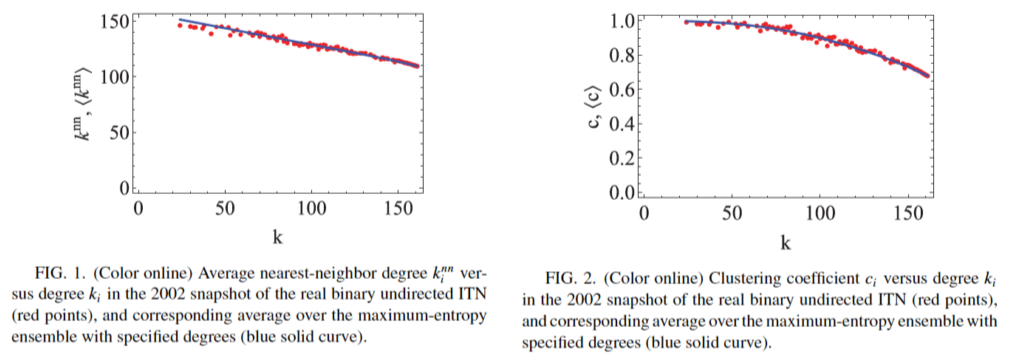
\includegraphics[width=0.6\textwidth]{picture/(44)world_trade_network_1.png}
\end{center}
The weighted configuration model explains well certain higher order metrics: disassortativity and decreasing clustering with degree.
\begin{center}
	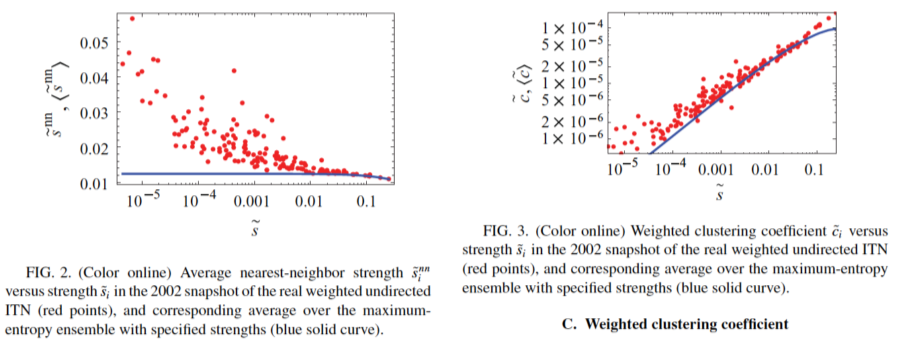
\includegraphics[width=0.6\textwidth]{picture/(45)world_trade_network_2.png}
\end{center}
\begin{myquote}
This important result implies that, even if we observe disassortativity in both cases (binary and weighted), we find that in the binary case this property is completely explained by the degree sequence, whereas in the weighted case it is not explained by the strength sequence. This has implications for economic models of international trade: While no theoretical explanation is required in order to explain why poorly connected countries trade with highly connected ones on a binary basis (once the number of trade partners is specified), additional explanations are required in order to explain the same phenomenon at a weighted level, even after controlling for the total trade volumes of all
countries.
\end{myquote}
\section{The interbank market}
Banks engage in establishing mutual credit relationships with varying maturities and collateral arrangements for purposes such as securing funding or utilizing excess liquidity. Interbank markets play a crucial role in enabling banks to manage and respond to specific liquidity shocks that may arise in the financial system.\\
The interbank market serves as the fundamental infrastructure or "plumbing" of modern financial systems. It facilitates the flow of funds and credit between banks, allowing them to meet their funding needs and address short-term liquidity imbalances efficiently.\\
Moreover, the interbank market is recognized as a significant conduit for the transmission of financial shocks within the financial system. Consequently, it holds substantial relevance in the assessment of systemic risk, which pertains to the potential instability or vulnerability of the entire financial system.
Let analyse sum property of network:
\begin{itemize}
	\item Very low connectivity: only $\sim 1\%$ of links are present
	\item Power law tailed distribution of in- and out- degree. Estimated exponent $\alpha \simeq 2 ÷ 3$
	\item The distribution of interbank exposures (node strenght) is also heavy-tailed.
	\item Low average distance between nodes
	\item A core periphery structure
	\item A disassortative mixing, i.e. the tendency of high degree nodes to connect with low degree nodes
	\item Small clustering
	\item An heterogeneous level of reciprocity
\end{itemize}
We would like applying maximum entropy approach to this network.\\
Many central banks do not require banks to report each credit or debit position, but only the aggregated assets and liabilities. In network terms this means that one knows only the node’s in- and out- strenght but not the degree, the adjacency matrix, and the weights of the individual links Assessing systemic risk through interbank market requires the knowledge of the interbank network. The aim in infer the structure of the interbank network from balance sheet data. Maxium entropy could help us in this aim.\\
The maximum entropy criteria assumes that banks spread their lending as evenly as possible. Finding the unknown entries of the liability matrix whose entries satisfy the algebraic and domain constraints and minimize the distance with the uniform vector, given the balance sheet constraints.\\
Distance can be quantified by the Kullback-Leibler divergence:
\[
D_{KL} (\vec{L}, \vec{Q}) = \sum_\alpha L_\alpha \ln \frac{L_\alpha}{Q_\alpha}
\]
\begin{myquote}
	To sum up, the evidence suggests that, in most cases, ME tends to underrate the impact of financial contagion. On the contrary, for high loss rates, ME may imply an overvaluation in the severity of
	contagion. (Mistrulli 2007)
\end{myquote}
Imposing only balance sheet constraints, maximum entropy performs bad in estimating systemic risk. This is due to the property of this network: it is very sparse. In models, systemic risk depends critically on the density of the interbank network.\\
If one knows the adjacency matrix of the interbank network, one can build more realistic maximum entropy ensembles.
Another way to consider interbank networks is considering interbank market as multiplex.\\
We need to distinguish among types of credit, analyzing either one specific segment (typically the unsecured overnight) or the aggregate of all the types of loans. Each node is a bank and each layer is a network representing one type of relation and the total network is the aggregation of all the layers of the multiplex.\\
During this discussion we include a wide range of collateralized (secured) / uncollateralized (unsecured) debt. We reclassified data to maturity:
\begin{itemize}
	\item overnight 
	\item short term ($t\leq$1Y)
	\item long term ($t >1$Y)
\end{itemize}
We obtain the following results:
\begin{itemize}
	\item After a decline of $25\%$ from 2008 to 2010, the 2012 consolidated volumes are close to those of 2008
	\item  The overnight interbank market is responsible for roughly one third of the total volume
	\item From 2010 we observe a decline in the unsecured short-term layer, mirrored by an increase of unsecured long-term lending. 
	\begin{itemize}
	\item Basel Liquidity Coverage Ratio significantly encourages borrowers to lengthen the maturity of their liabilities. 
	\item Shift of interbank lending from a money market, risk-free activity to a credit-intensive one, as a result of repeated bank failures and seizures during the financial crisis.
	\end{itemize}
	\item The drop in secured interbank lending is mostly due to regulatory incentives towards centrally cleared as opposed to over-the-counter repurchase agreements, which turns
	into increasing costs of establishing bilateral lending agreements.
	\item Topology quite stable in time
	\item Layers pretty different one from each other 
	\item The overnight layer is topologically very similar to the total network, essentially
	because all banks are incolved in the overnight market
	\item The estimated values of the tail exponent $\alpha$ are remarkably stable across layers and over time. The range of values of $\alpha$ is $[1.8, 3.5]$
	\item The core is a subset of nodes which are maximally connected with other core members, while the periphery is the complementary subset made of nodes with no reciprocal
	connections but only with the core.
	\item The correlation between two partitions across different time periods ranges from 0.84 to 0.97. The correlation between different layers in the same period is generally lower, ranging between 0.31 (overnight vs secured short-term in 2012) and 0.79.
	\item Overnight and unsecured short term display the largest correlation with total asset, while this is lower for secured short term and unsecured long term.
	\item The large heterogeneity of bank size drives most of the topological structure of interbank market
\end{itemize}
Summarize:
\begin{itemize}
	\item The scale free behavior (i.e. large heterogeneity) of degree is a generic property 
	\item Different level of correlation between degree (number of creditors) and weight (amout of credit) in different layers
	\item The high value of reciprocity (in degree but not in weight) might be due to the fact that many banks still hold bilateral deposit accounts at other banks for the settlement of retail payments (see also later)
	\item Most layers display a disassortative behavior 
	\item The low value of clustering (comparing with other studies) is likely due to the use of
	consolidated data
\end{itemize}
Let use Maximum Entropy Principles, we investigate the following ensembles:
\begin{itemize}
	\item Directed Binary Configuration model (DBCM), where the in- and out-degree of each node is preserved \item Reciprocal Configuration Model (RCM), where also the number of reciprocated relations of each node is preserved 
	\item Directed Weighted Configuration Model (DWCM), where we preserve the in- and
	out-strenght, as well as the in- and out-degree, of each node
\end{itemize}
As higher order properties:
\begin{itemize}
	\item Number of reciprocated links R 
	\item Assortativity Number of triangles T
	\item Triadic structure, i.e. third order motifs
\end{itemize}
The results show:
\begin{itemize}
	\item Real reciprocity is higher than what expected by taking into account in- and out-degree 
	\item Largest strong and weak components are larger in real data
	\item Number of triangles is smaller in real data than in the model
\end{itemize}
From this work, we obtain the folloqing conclusions:
\begin{itemize}
	\item Different layers of the interbank network have several topological and metric properties which are layer-specific, while other properties seem to be more “universal”
	\item The topology of the total interbank market is closely mirrored by the one of the overnight market, while both are little informative about other layers; 
	\item Higher order topological properties, such as triadic structures or reciprocated links, are explained by random models in some layers;
	\item Random models that jointly consider topological and metric properties provide a close representation of the metric properties of different layers, as long as the calibration of the model is layer-specific
	\item From a policy perspective:
	\begin{itemize}
		\item The heterogeneity of layers reduce the probability that the failure of a node (bank) propagates in one of its neighbor 
		\item However the heterogeneity could speed up the propagation of cascades, because it makes the system more (long range) connected 
		\item The nowledge on the overnight is little informative on the network structure in the other layers: systemic risk underestimation If policymakers and researchers alike were to target a specific segment of the interbank network, they should be careful in adopting an analytical framework based on the
		overall features of the network
	\end{itemize}
\end{itemize}
\newpage
\section{Systemic risk}
\begin{mydefinition}[Systemic risk]
	Systemic risk is the risk of collapse of an entire financial system or entire market, as opposed to risk associated with any one individual entity, group or component of
	a system.
\end{mydefinition}
Financial systemic risk is mediated by a set of interconnected networks. There are at list two channels of systemic risk propagation:
\begin{itemize}
	\item Common esposures and fire sale spillvoers
	\item Illiquidity cascades in the interbank network
\end{itemize}
It is important understand what is the role of network structure and how network change in response to exceptional events and which data are necessary to assess systemic risk.\\
Fire sales spillovers due to assets’ illiquidity and common portfolio holdings are definitely one of the main drivers of systemic risk. Shared investments create a significant overlap of portfolios between couples of financial institutions and fire sales move prices due to the finite liquidity of assets and to market impact. Finally, leverage management amplifies such feedbacks.\\
Let consider the following setting:
\begin{mysetting}[Systemic risk metrics: Vulnerability and Systemicness]
	\begin{itemize}
		\item A system composed by $N$ banks and $K$ asset classes. 
		\item Matrix $\textbf{X}$ of portfolio holdings, whose element $X_{n,k}$ is the dollar-amount of $k$-type assets detained by bank $n$.
		\item Matrix of portfolio weights is:
		\[
		W_{n,k}(\mathbf{X}) = \frac{X_{n,k}}{\sum_{k'=1}^{K} X_{n,k'}}
		\]
		\item Discretization of $X_{n,k}$, in such a way that the matrix $X$ belongs to the space $\mathbb{N}^{N\times K}$ of $N \times K$ integer valued matrices
	 \end{itemize}
\end{mysetting}
The total asset size $A_n$ of the $n$-th bank and the total capitalization $C_k$ of the k-th asset class are:
\[
A_n(\mathbf{X}) = \sum_{k=1}^{K} X_{n,k} \qquad C_k(\mathbf{X}) = \sum_{n=1}^{N} X_{n,k}
\]
The rectangular matrix $\mathbf{X}$ can be naturally associated to a bipartite network, while the two quantities $A_n, C_k$ are the strength sequences for the two sets of nodes.\\
We define the leverage of bank $n$ as:
\[
B_n = \frac{A_n - E_n}{E_n}
\] where $E_n$ is the equity.\\
Each asse class is characterized by an illiquidity parameter $\ell_k$ defined as the return per dollar of net purchase of asset k.\\
Given an asset shock described by the $K$ dimensional vector $F_1 = -\mathbf{\varepsilon} = (-\epsilon_1,\ldots,\varepsilon_k) $, we define:
\begin{itemize}
	\item \textbf{Aggregate vulnerability ($AV$)} as the percentage of aggregate bank equity that would be wiped out by bank deleveraging if there was a shock to asset returns. 
	\item \textbf{Bank systemicness} ($S_n$) as the contribution of bank $n$ to aggregate vulnerability. \item \textbf{Bank’s indirect vulnerability} $IV_n$ as the impact of the shock on its equity through the deleveraging of other banks
\end{itemize}
We can derivare the metrics for systemic risk:
\begin{mydefinition}[Metrics systemic risk]
	\begin{itemize}
		\item Banks returns given asset returns, $R_1 = WF_1$
		\item Banks sell asset to return to leverage targets, then asset change of banks is $A_1BR_1$
		\item Proportional rebalancing of banks, asset purchase by all banks is $\phi = W'A_1BR_1$
		\item Fire sales generate (linear) price impact, $F_2 = L\phi$
		\item Effect on banks of fire sales, $R_2 = WF_2 = WL\phi = (WLW'BA_1)R_1$
		\item Aggregate vulnerability:
		\[
		AV = \frac{1'A_1 \cdot WLW'BA_1WF_1}{E_1}
		\]
		\item Bank systemicness, its contribution to AV:
		\[
		S_n = \frac{1'A_1 \cdot WLW'BA_1 \delta_n \delta'_nWF_1}{E_1}
		\]
	\end{itemize}
\end{mydefinition}
Using Maximum and Cross Entropy, we can conclude that:
\begin{itemize}
	\item We proposed a Maximum and Cross Entropy to reconstruct an unknown network from partial information.
	\item We find that the detailed knowledge of the portfolio (i.e. network) composition is unnecessary to estimate systemic risk due to fire sales spillover.
	\item Maximum Entropy could be used to identify significant changes in the systemicness of individual banks, groups of banks, or of the whole system
\end{itemize}
\section{Exponential Family of Distributions}
\begin{mydefinition}[Exponential Family of Distribution]
	Given a random vector $\mathbf{Y} = (Y_1,\ldots,Y_n)$, it follows a distribution of an exponential family if its probability density function can be written as:
	\[
	P(\mathbf{Y| \theta}) = \frac{\exp(\sum_s \theta_s h_s(\mathbf{Y}))}{\mathcal{K}(\theta) \mathcal{H}(\mathbf{Y})}
	\]
\end{mydefinition}
where $\theta = (\theta_1,\ldots, \theta_s)$ is a vector of parameters and $h_s(\mathbf{Y})$ is a set  of statistics, this is suffeicent for parameter $\theta_s$. The function $\mathcal{K}(\theta)$ and $\mathcal{H}(\mathbf{Y})$ are normaling factors. Given explicit form for $P(\mathbf{Y})$, we can estimate $\theta$ throug MLE.\\
EFDs naturally arises when constructing Maximum Entropy distributions. Assume the variables are discrete, the problem is:
\[
\max_{\{P\}} \left(- \sum_i P_i \ln P_i\right) \qquad \text{s.t.} \qquad \sum_i P_i = 1 \qquad \sum_i P_ih_i^s = \bar{h}^s
\].
This problem can be used trough Lagrange multipliers:
\[
P_j = \frac{\exp(-\sum_s \theta_s h_j^s)}{\sum_j \exp (-\sum_s \theta_sh_j^s)}
\]
This is  a distribution of the exponential family.\\
We can apply this to network, taking $h_s(\mathbf{A})$ as network metrics. The complitcated task is to compute the denominator.
\subsection{Latent node-specific parameter models}
Models with latent node-specific parameters are flexible network formation mechanisms, able to generate a wide range of structural features, where each node $i$ is associated with a vector of parameters $\theta_i$.\\
Links are formed between nodes with a probability:
\[
\mathbb{P}(A_{ij} = 1) = f(\theta_i,\theta_j)
\]
we call $f(\cdot)$ link function.\\
The configuration model can be seen as a latent parameters model where the $\theta$s are continuous variables associated with the degree:
\[
\mathbb{P}(A_{ij}= 1| \theta_i,\theta_j) = \frac{1}{1 + e^{-(\theta_i + \theta_j)}}
\] 
In Stochastic Block Model, the $\theta$s are discrete variables identifying the group or block the node belong to.\\
The Maximum Likelihood Estimate of the parameters $\theta$ for the fitness model described by probability distribution:
\[
\mathbb{P}(\mathbf{A}|\mathbf{\theta}) = \prod_{i,j>1}\frac{e^{A_{ij}(\theta_i + \theta_j)}}{1 + e^{\theta_i + \theta_j}}
\]
can be obtained by minimizing the likelihood function:
\[
\ell (\mathbf{\theta}) = - \sum_i \theta_ik_i^* + \sum_{i,j>i} \log \left(1 + e^{\theta_i + \theta_j}\right)
\]
with $k^*_i$ the observed degree of node $i$.\\
\begin{mydefinition}[Polytope of degree]
	The polytope of degree sequences which is defined as the convex hull of all possible degree sequence:
	\[
	P_N \equiv \text{convhull} (\{\mathbf{K}(G), G \in \mathcal{G}_N\})
	\]
\end{mydefinition}
\begin{mytheorem}[Existence of the solution of the MLE (Rinaldo et al. 2013)]
	Let $G^\ast \in \mathcal{G}_N$ be the observed graph in the network ensemble. The MLE exists if and only if $\mathbf{k}^\ast(G^\ast) \in \text{int}(P_N)$ 
\end{mytheorem}
\begin{mydefinition}[Stable Set]
	Let $G = (V,E)$ be a graph. A subset $W\subseteq V$ is a stable set if the subgraph of $G$ induced by $W$ is an adgeless graph
\end{mydefinition}
\begin{mydefinition}[Clique]
	Let $G = (V,E)$ be a graph. A subset $W\subseteq V$ is a clique if the subgraph of $G$ induced by $W$ is a complete graph
\end{mydefinition}
\newpage
\begin{mytheorem}[Existence and property of MLE solution (Rinaldo et al 2013)]
Let $\mathbf{k}$ be the degree sequence of a graph $G = (V,E)$ with $|V| =N$, that is on the boundary of $P_N$. Then either $k+i = 0$ or $k+i = N-1$ dor some $i \in \{1,\ldots,N\}$, or there exist nonempty and disjoint subsets $S$ and $T$ of $\{1,\ldots,N\}$ s.t:
\begin{itemize}
	\item $S$ is a clique of $G$;
	\item $T$ is a stable set of $G$;
	\item every vertex in $S$ is adjacent to every vertex in $(S \cup T)^c$ in $G$;
	\item no vertex of $T$ us adjacent to any vertex of $(S\cup T)^c$ in $G$
\end{itemize}
\end{mytheorem}
\begin{center}
	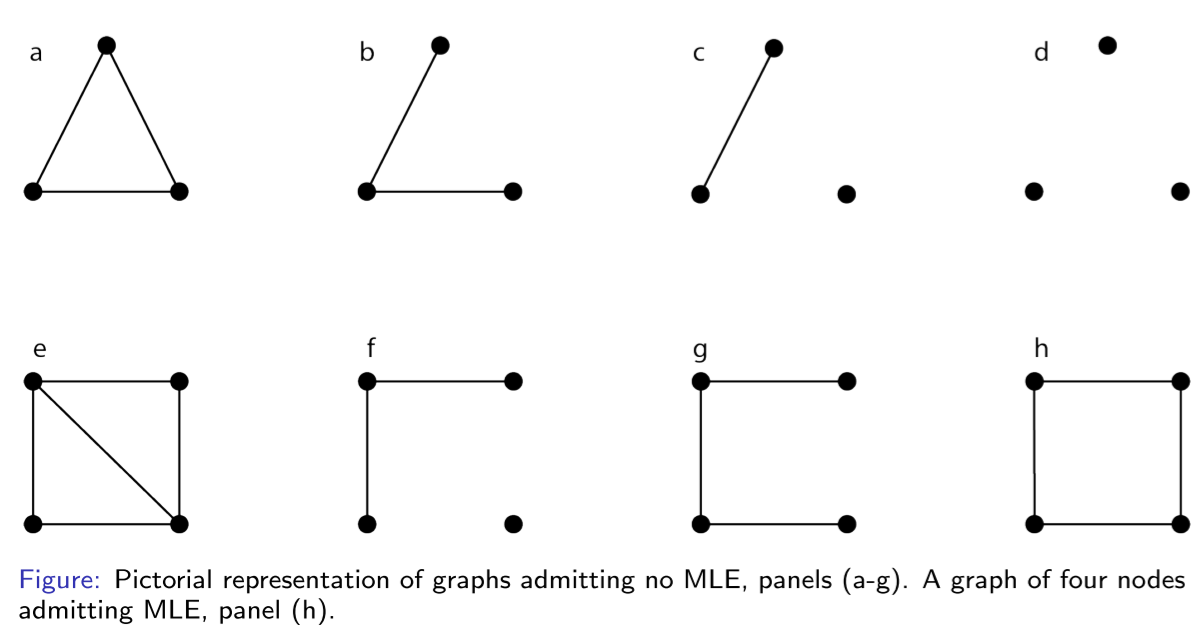
\includegraphics[width=0.6\textwidth]{picture/(46)MLE_admitting.png}
\end{center}
In general it is not a trivial task to characterize the convex hull $P_N$ for a given $N$. In the asymptotic limit $N\to \infty$ it holds:
\begin{mytheorem}[Asymptotic behaviour of MLE solutions Chatterjee et al. (2011)]
	Let be $G^* \in \mathcal{G}_N, \mathbf{k}^\ast(G^\ast)$ the degree sequence of $G^\ast$ and $L \equiv \max_{1\leq i \leq N} |\theta_i|$. Then, there is a constant $C(L)$ depending only on $L$ such that with probability at least $1- C(L)N^{-2}$, there exists a unique solution $\mathbf{\hat{\theta}}$ of the MLE, which satisfie:
	\[
	\max_{1\leq i \leq N} |\hat{\theta}_i - \theta_i| \leq C(L) \frac{\log N}{N}
	\]
\end{mytheorem}
From this theorem we noticed that:
\begin{itemize}
	\item The number of graphs having degree sequence on the boundary of $P_N$ is increasing with $N$,however the probability of suchgraphs over the ensemble is vanishing as $N$ grows.
	\item If there exists the MLE of the fitness model, Chatterjee et al. (2011) have proved the uniqueness of the solution
\end{itemize}
There is a fast algorithm for computing the MLE if it exists, which is referred as Iterative Proportional Fitting Procedure (IPFP).\\
Let be $\varphi: \mathbb{R}^N \to \mathbb{R}^N$ a vector-valued function whose generic $i$- component is:
\[
\varphi_i(\mathbb{\theta})\equiv \log k_i^\ast - \log \sum_{j\neq i} \frac{e^{\theta_j}}{1 + e^{\theta_i + \theta_j}}
\]
If the MLE exists, then it is the fixed-point of the function $\varphi$.
\begin{mytheorem}[Unique solution MLE Chatterjee et al. 2011]
Let be $G^\ast \in \mathcal{G}_N$, $\mathbf{k}^\ast$ the degree sequence of $G^\ast$, and assume there exists the solution $\hat{\theta}$ of the maximum likelihood problem. Then, $\hat{\mathbf{\theta}}$ is the fixed-point ofthe function $\varphi$. Then, $\mathbf{\theta}_{t +1}$ converges to $\mathbf{\hat{\theta}}$ geometrically fast in the $L^\infty$ norm where the rate depends only on $|\hat{\theta}|_{\infty}, |\hat{\theta_0}|_{\infty}|$. In particular, $\hat{\theta_0}$ must be the unique solution of the system ofnonlinear equations . Conversely, if the maximum likelihood problem does not have a solution, then the sequence $\{\theta_t\}$ must have a divergent subsequence.
\end{mytheorem}
\section{Temporal networks}
There are essentially two methods to build statistical models for temporal networks:
\begin{itemize}
	\item Assume that some network observables are time varying. One can specify:
	\begin{itemize}
		\item The dynamical equation of the observables
		\item The expectation of some statistics of observables at different times
	\end{itemize}
\item Assume that the network is formed because of latent variables. One can specify:
\begin{itemize}
	\item The dynamical equation of the latent variables
	\item Filter the dynamics of the latent variables
\end{itemize}
\end{itemize}
Many networks are inherently dynamic as links are created and destroyed through time:
\begin{itemize}
	\item Preferential relations between nodes tend to preserve past links (If we were friends yesterday we will be friend today)
	\item Node specific properties can drive the evolution of the network topology (Two social persons are more likely to be friend)
\end{itemize}
In general, the dynamics will be a combination of the two types of mechanisms.
\subsection{DAR(p) model}
We model the tendency of a link that does (or does not) exist at time $t-1$ to continue existing (or not existing) at time $t$. We define Discerete AutoRegressive DAR(1) model as:
\[
\mathbb{P}(\mathbf{A}^t | \mathbf{A}^{t-1}, \bm{\alpha},\bm{\chi}) = \prod_{i\neq j} \underbrace{\alpha_{ij}\delta_{A^t_{ij}A_{ij}^{t-1}}}_{\substack{\text{Copying the last observation} \\ \text{with the probability }\alpha_{ij}}} + (1-\alpha_{ij})\chi_{ij}^{A_{ij}^t} (1 - \chi_{ij})^{1 - A_{ij}^t}
\]
One indpendent process per link and the larger is $\alpha_{ij}$ the more persistent is the link between $i$ and $j$.
\begin{mydefinition}[DAR(p) model]
	\begin{align*}
		&X_n = V_n X_{n-A_n}  + (1-V_n)Z_n\\
		Z_n \sim  \Xi, \qquad V_n \sim &\mathcal{B}(1,\chi), \qquad P(A_n = i) = \phi_1, \qquad \sum_{i=1}^P \phi_i = 1
	\end{align*}
\end{mydefinition}
The autocorrelation function $\rho_k = Corr(X_n, X_{n+k})$ satisfies:
\[
\rho_k = \chi \sum_{i =1}^p \phi_i \rho_{k-i} \quad k\geq 1
\]
it describes a AR process.\\
Model predictor conditional on $\Omega_{n-1} = \{ X_{n-1},\ldots, X_{n-p}\}$:
\[
\hat{X}_{n+s} \equiv \expected{X_{n+s}| \Omega_{n-1}} = \chi \sum_{i=1}^{p}\phi_iY_{n+s-i} + \expected{Z}(1- \chi), \quad Y_{n+s-i} = \begin{cases}
	\hat{X}_{n+s-i} & \text{for }i\leq s\\
	 X_{n+s-i} & \text{for }i> s\\
\end{cases}
\]
We have:
\[
\mathbb{P}(\mathbf{A}^t | \mathbf{A}^{t-1}, \bm{\alpha},\bm{\chi}) = \prod_{i,j>i} \alpha_{ij}\delta_{A^t_{ij}A_{ij}^{t-1}} + (1-\alpha_{ij})\chi_{ij}^{A_{ij}^t} (1 - \chi_{ij})^{1 - A_{ij}^t}
\]
we noticed that:
\begin{itemize}
	\item Copying from the past with probability $\alpha_{ij}$, otherwise a Bernoulli trial with probability of success $\chi_{ij}$.
	\item The larger is $\alpha_{ij}$, the more persistent is the link.
	\item Fully specified by the $2 {N \choose 2}$ parameters $\{\bm{\alpha}, \bm{\chi}\}_{i=1,\ldots,N;j > i}, \alpha_{ij} \in [0,1]$ and $\chi_{ij} \in [0,1]$
	\item Is a first order process of the class of DAR(p) models
\end{itemize}
\subsection{Vectror DAR (VDAR(1)) model}
The VDAR(1)  model describes the dependence structure of a set of binary random variables which has Markov property and Bernoulli marginal distribution.\\
Given $N$ binary variables $\mathbf{X}_t \equiv \{X_t^i\}_{i =1,\ldots,N}$ with $X_t^i \in \{0,1\}$, the VDAR(1) process describes the evolution of $X_t^i$ as:
\[
X_t^i =V_t^i X_{t-1}^{A_t^i} + (1-V_t^i)Z_t^i
\]
with $V_t^i \sim \mathcal{B}(\nu_i)$ a Bernoulli random variable with parameter $\nu_i \in [0,1]$, $A_t^i \sim \mathcal{M}(\lambda_{i1},\ldots,\lambda_{iN})$ a multinomial random variable taking integer value in $\{1,\ldots,N\}$, with parametera $\lambda_{i1},\ldots,\lambda_{iN}$ s.t. $\sum_{j =1}^N \lambda_{ij} =1$ and $Z_t^i \sim \mathcal{B}(\chi_i)$ with $\chi_i \in [0,1]$.\\
The VDAR(1) process describe the copying from the past: with probability $\nu_i$, $X_t^i$ is copied from the past and with probability $X_t^i$ is equal to $X^j_{t-1}$; otherwise $X^j_{t}$ is not copied ans is sampled according to a Bernoulli marginal with probability $\chi_i$. Model is formalized bu the transition probability:
\[
p_{VDAR}(\mathbf{X}_t | \mathbf{X}_{t-1}; \bm{\pi}) = \prod_{i=1}^N \left[\nu_i \left(\sum_{j =1}^N \lambda_{ij}\delta_{X^i_t,X^i_{t-1}}\right) + (1- \nu_i)(\chi_i)^{X_t^i}(1- \chi_i)^{1 - X^i_t}\right]
\]
where $\bm{\pi} = \{\{v_i\},\{\lambda_{ij}, \{\chi_{ij}\}\}\}_{i,j =1,\ldots,N}$
\subsection{Temporal Exponential Random Graph (TERGM)}
One can instead fix the expectation of some statistics at different times and invoke Maximum Entropy, we can extend ERG to the temporal case.\\
A TERGM describes a stationary dynamics via the following dependencies among the links:
\[
\log P\left(\bm{Y}^{(t)}|\theta, \bm{Y}^{(t-K)},\ldots, \bm{Y}^{(te)}\right) = \sum_s \theta_s h_s \left(\bm{Y}^{(t-K)},\ldots, \bm{Y}^{(t)}\right) - \log(\mathcal{K}(\theta))
\]
The model can be estimated via Maximum Likelihood.\\
One could consider Markov chains ($K$ =1) and as statistics the density and number of preserved links:
\begin{align*}
	&\log P \left(\bm{Y}^{(t)}| \theta, \bm{Y}^{(t-1)},\bm{Y}^{(t)}\right) =\\
	& \theta_1 \sum_{i>j} Y_{ij}^{(t)} + \theta_2 \sum_{i>j} [Y_{ij}^{(t)}Y_{ij}^{(t-1)} + (1- Y^{(t)}_{ij})(1- Y_{ij}^{(t-1)})] - \log (\mathcal{K} (\theta))
\end{align*}
This model is mathematically equivalent to the DAR(1) model. An analogous equivalence holds for non-Markovian DAR(p) models and TERGM.\\
The KIM describes the time evolution of a set of binary variables $s(t) \in \{-1, 1\}^N$ for $t =1,\ldots,T$ typically called "spins", which can influence each other through a time lagged interaction.\\
The model is Markovian with synchronous dynamics, characterized by transition probability:
\[
p(s(t+1)| s(t), x(t); \beta, \Theta) = \frac{e^{\beta \sum_i s_i(t+1)g_i(t)}}{Z(t)}
\]
where $J$ is a $N \times N$ interaction matrix, the $N-$ dimensional vector $h$ and the $N\times K$ matrix $b$ characterize the interaction with external covariates $x(t) \in \mathbb{R}^k$, and $Z(t)$ is a normalizing costant (partition function), $\beta$ is a parameter that determines the amount of noise in dynamics. The quantity $g_i(t) \equiv \sum_j J_{ij}s_j(t) + h_i + \sum_k b_{ik}x_k (t)$ is called the effective spin.
\begin{mytheorem}[Equivalence between Ising Model and VDAR(1) (Campajola et al. JSTAT, 2021)]
	The Kinetic Ising Model is equivalent to the VDAR(1) model if and only if $J_{ij} \geq 0, \quad \forall i,j$
\end{mytheorem}
Let analyse the fitness. Each node $i$ is characterized by a quantity $\theta_i^t$ ,i.e. the node fitness.We assume that it follows an AR(1) process:
\[
\theta_t^i = \phi_{0,i} + \phi_{1,i}\theta_i^{t-1} + \epsilon^t_i
\]
$\phi_{0,i} \in \mathbb{R},|\phi_{1,i}|<1$ and $\epsilon_i^t\sim NID(0,\sigma_i)$ with $\sigma_i > 0$.\\
We define the link probability at time $t$ as:
\[
\mathbb{P}(A^t_{ij} =1 |\theta_i^t, \theta_j^t) = \frac{1}{1 + e^{- (\theta_i^t + \theta_j^t)}}
\]
The larger $\theta_i^t$ is, the larger is the probability for all links incident to node $i$ at time $t$.\\
TGRG describes the process of link rewiring at each time step according to the dynamic fitness of the nodes.\\
Mixture the two linking mechaninsm we find a model that:
\begin{itemize}
	\item Copying from the past with probability $\alpha_{ij}$ and a time evolving marginal described by the dynamic fitness model with probability $1-\alpha_{ij}$.
	\item $\alpha_{ij}$ disentangles the two mechanisms for each link.
\end{itemize}
General comments:
\begin{itemize}
	\item We introduce new statistical models of temporal networks. 
	\item We generalize the fitness model to the dynamic case. TGRG describes how the network topology (degree) changes in time.
	\item We model link stability via the Discrete AutoRegressive mechanism. Link persistence is statistically associated with preferential linkage.
	\item In e-MID, DAR-TGRG disentangles preferential and random trading.
	\item Link prediction in temporal networks by accounting for both link stability and
	time-varying topologies
\end{itemize}
\section{Time-varying parameter models}
Following Cox (1981), we divide time-varying parameter models into two classes:
\begin{itemize}
	\item \textbf{Parameter-driven models:}Parameters evolve based on idiosyncratic innovations (e.g. Stochastic Volatility, Temporal fitness, etc.)
	\item \textbf{Observation-driven model:}Parameters evolve based on a nonlinear function of past observations (e.g. GARCH)
\end{itemize}
\begin{mydefinition}[Generalized Auto-regressive Score-driven (GAS) models]
We define GAS model as:
\begin{align*}
	y_t = g(f_t,u_t), \quad u_t \sim p(u|\theta) \quad i.i.d\\
	f_{t+1} =\omega + \alpha s(y_t,f_t) + \beta f_t
\end{align*}
where:
\begin{itemize}
	\item $\omega, \alpha, \beta, \theta$ are time=invariant scalar parameter
	\item $s(y_t,f_t) = \nabla(y_y,f_t) \cdot S(f_t)$ is a scaled-score:
	\begin{align}
	& \nabla(y_t,f_t) = \frac{\partial \log p(y_t | f_t)}{\partial f_t}\\
	& S(f_t) = \mathcal{I}^{-1}_{t|t-1} = \mathbb{E}^{-a}[\nabla (y_t,f_t) \nabla'(y_t,f_t)|\mathcal{F}_{t-1}]
	\end{align}
with $a = 0,1,1/2$
    \item $s(y_t,f_t)$ can be linear, non-linear or invariant in $f_t$
    \item The update of Dynamic Conditional Score-driven models is optimal according to Kullback-Leibler distance.
\end{itemize}
\end{mydefinition}
\subsection{Financial voaltility}
Financial log-prices can be described as a random walk. However it is clear that the diffusion rate of the random walk (the volatility)is not constant, but fluctuates in time with a very slowly decaying autocorrelation. Notice that volatility cannot be observed but is a latent variable. We can adopt two approaches:
\begin{itemize}
	\item Write a dynamical equation for the volatility
	\item Try to filter the volatility from the time series
\end{itemize}
We can apply GAS model for price return: consider a stochastic volatility model $r_t \equiv y_t = \sigma_t \epsilon_t$ with $\epsilon_t \sim \mathcal{N}(0,1)$. In this case we choose $f_t = \sigma_t^2$ and:
\[
\frac{\partial \log p(y_t| f_t, \mathcal{F}_{t-1};\Theta)}{\partial f'_t} = - \frac{1}{2 \sigma^2_t} + \frac{y_t^2}{2 \sigma_t^4}
\]
hence:
\[
\sigma^2_{t+1} = \omega + B \sigma_t^2 + \frac{AS(\sigma_t)}{2}\left[\frac{y_t^2 - \sigma^2_t}{\sigma^4_t}\right]
\]
If $y^2_t\gg \sigma_t^2 (y_t^2 \ll \sigma_t^2)$ the new $\sigma^2_{t+1}$ eill be larger (smaller) than $\sigma_t^2$. Choosing $S$ as the inverse of the information matrix:
\[
- \expected{\frac{\partial^2 \log p}{\partial \sigma^2}} = \frac{1}{2 \sigma^4}
\]
thus:
\[
\sigma^2_{t+1} = \omega + B \sigma_t^2 + A(y_t^2 - \sigma_t^2) = \omega + \alpha y_t^2 + \beta \sigma_t^2
\]
that is exactly a GARCH model.\\
Other popular econometric models as Multiplicative Error Model (MEM), Autoregressive Conditional Duration (ACD), Autoregressive Conditional Intensity (ACI) can be casted as special cases of the GAS.\\
We can use Garch model as filter:
\[
\sigma_t^2 = \omega + \alpha r_{t-1}^2 + \beta \sigma^2_{t-1}
\]
For the general ERGM, the elements of the score take the form:
\[
\nabla^{(t)}_s (\theta) = \frac{\partial \log P \left(\mathbf{A}^{(t)}|\theta\right)}{\partial \theta_s} = h_s \left(\mathbf{A}^{(t)}\right) - \frac{\partial \log \mathcal{K}(\theta)}{\partial \theta_s}
\]
It follows that the vector of time-varying parameters evolves according to:
\[
\theta^{(t+1)} = w + \bm{\beta}\theta^{(t)} + \bm{\alpha}\mathbf{S^{(t)}}\nabla^{(t)} \left(\theta^{(t)}\right)
\]
When the sequence of networks $\left\{\mathbf{A}^{(t)}\right\}^T_{t = 1}$ is observed, the static parameter $(\bm{w,\beta,\alpha})$ that best fit the data can be estimated via MLE.\\
Despite simple in principle, working with (T)ERGM different from the fitness model presents two main difficulties:
\begin{itemize}
	\item \textbf{Computability:} The computation of the normalization factor $\mathcal{K}(\theta) $is prohibitive
	\item \textbf{Degeneracy: }An ERGM is degenerate if it concentrates a large portion of its probability on a small set of configurations, typically the uninteresting graphs that are completely connected or void of links. Example: statistic equal to the number of triangles.
\end{itemize}
\subsection{Maximum Pseudo Likelihood Estimation}
Given an ERGM, the change statistic for the link between node $j$ and $i$,associated with network statistic $h_s$ is:
\[
\delta^s_{ij} = h_s(\mathbf{A}_{ij}^+)-h_s(\mathbf{A}_{ij}^-)
\]
where $\mathbf{A}_{ij}^+$ is a matrix s.t $A^+_{ij} =1$ and it is equal to $\mathbf{A}$ in all other elements, while $\mathbf{A}_{ij}^-$ has  $A^-_{ij} =0$ and it is equal to $\mathbf{A}$ in all other entrie.\\
Given these definitions, the pseudo-likelihood reads:
\[
PL(\mathbf{A}|\theta) = \prod_{ij} \pi_{ij}^{A_{ij}} (1- \pi_{ij})^{(1 - A_{ij})}
\]
where $\pi_{ij} = (1 + e^{-\sum_s \theta_s \delta^s_{ij}})^{-1}$.\\
THe maximum pseudo-likelihood estimates correpsonf to the paramter values $\theta$ that maximize the pseudo-likelihood.\\
Let give now the final conclusion:
\begin{itemize}
	\item Flexible class of models for temporal networks 
	\begin{itemize}
		\item Different mechanisms for link creation: latent node variable, copying past links, etc. 
		\item Different network statistics preserved on average: degree, number of common neighbors, etc. \item Stationary and non stationary dynamics 
		\item Related to Maximum Entropy approach
	\end{itemize}
	\item Clear improvement on link prediction as compared with forecast based on models of the observed links.
	\item Testing whether some parameter/statistic is constant 
	\item Even if the data generating process is generic, the SD-ERGM is a very effective filter of the dynamics of the latent variables or parameters.
\end{itemize}